\documentclass{sigchi}

% Use this section to set the ACM copyright statement (e.g. for
% preprints).  Consult the conference website for the camera-ready
% copyright statement.

% Copyright
\CopyrightYear{2020}
%\setcopyright{acmcopyright}
\setcopyright{acmlicensed}
%\setcopyright{rightsretained}
%\setcopyright{usgov}
%\setcopyright{usgovmixed}
%\setcopyright{cagov}
%\setcopyright{cagovmixed}
% DOI
\doi{https://doi.org/10.1145/3313831.XXXXXXX}
% ISBN
\isbn{978-1-4503-6708-0/20/04}
%Conference
\conferenceinfo{CHI'20,}{April  25--30, 2020, Honolulu, HI, USA}
%Price
\acmPrice{\$15.00}

% Use this command to override the default ACM copyright statement
% (e.g. for preprints).  Consult the conference website for the
% camera-ready copyright statement.

%% HOW TO OVERRIDE THE DEFAULT COPYRIGHT STRIP --
%% Please note you need to make sure the copy for your specific
%% license is used here!
% \toappear{
% Permission to make digital or hard copies of all or part of this work
% for personal or classroom use is granted without fee provided that
% copies are not made or distributed for profit or commercial advantage
% and that copies bear this notice and the full citation on the first
% page. Copyrights for components of this work owned by others than ACM
% must be honored. Abstracting with credit is permitted. To copy
% otherwise, or republish, to post on servers or to redistribute to
% lists, requires prior specific permission and/or a fee. Request
% permissions from \href{mailto:Permissions@acm.org}{Permissions@acm.org}. \\
% \emph{CHI '16},  May 07--12, 2016, San Jose, CA, USA \\
% ACM xxx-x-xxxx-xxxx-x/xx/xx\ldots \$15.00 \\
% DOI: \url{http://dx.doi.org/xx.xxxx/xxxxxxx.xxxxxxx}
% }

% Arabic page numbers for submission.  Remove this line to eliminate
% page numbers for the camera ready copy
% \pagenumbering{arabic}

% Load basic packages
\usepackage{balance}       % to better equalize the last page
\usepackage{graphics}      % for EPS, load graphicx instead 
\usepackage[T1]{fontenc}   % for umlauts and other diaeresis
\usepackage{txfonts}
\usepackage{mathptmx}
\usepackage[pdflang={en-US},pdftex]{hyperref}
\usepackage{color}
\usepackage{booktabs}
\usepackage{textcomp}

% Some optional stuff you might like/need.
\usepackage{microtype}        % Improved Tracking and Kerning
% \usepackage[all]{hypcap}    % Fixes bug in hyperref caption linking
\usepackage{ccicons}          % Cite your images correctly!
% \usepackage[utf8]{inputenc} % for a UTF8 editor only

% If you want to use todo notes, marginpars etc. during creation of
% your draft document, you have to enable the "chi_draft" option for
% the document class. To do this, change the very first line to:
% "\documentclass[chi_draft]{sigchi}". You can then place todo notes
% by using the "\todo{...}"  command. Make sure to disable the draft
% option again before submitting your final document.
\usepackage{todonotes}

%
\usepackage{gensymb}
%

% Paper metadata (use plain text, for PDF inclusion and later
% re-using, if desired).  Use \emtpyauthor when submitting for review
% so you remain anonymous.
\def\plaintitle{CollaboVR: A Reconfigurable Framework for Multi-user to Communicate in Virtual}
\def\plainauthor{Zhenyi He, Ken Perlin}
\def\emptyauthor{}
\def\plainkeywords{Virtual Reality; free-hand drawing; computer-supported collaborative work.}
\def\plaingeneralterms{Documentation, Standardization}

% llt: Define a global style for URLs, rather that the default one
\makeatletter
\def\url@leostyle{%
  \@ifundefined{selectfont}{
    \def\UrlFont{\sf}
  }{
    \def\UrlFont{\small\bf\ttfamily}
  }}
\makeatother
\urlstyle{leo}

% To make various LaTeX processors do the right thing with page size.
\def\pprw{8.5in}
\def\pprh{11in}
\special{papersize=\pprw,\pprh}
\setlength{\paperwidth}{\pprw}
\setlength{\paperheight}{\pprh}
\setlength{\pdfpagewidth}{\pprw}
\setlength{\pdfpageheight}{\pprh}

% Make sure hyperref comes last of your loaded packages, to give it a
% fighting chance of not being over-written, since its job is to
% redefine many LaTeX commands.
\definecolor{linkColor}{RGB}{6,125,233}
\hypersetup{%
  pdftitle={\plaintitle},
% Use \plainauthor for final version.
%  pdfauthor={\plainauthor},
  pdfauthor={\emptyauthor},
  pdfkeywords={\plainkeywords},
  pdfdisplaydoctitle=true, % For Accessibility
  bookmarksnumbered,
  pdfstartview={FitH},
  colorlinks,
  citecolor=black,
  filecolor=black,
  linkcolor=black,
  urlcolor=linkColor,
  breaklinks=true,
  hypertexnames=false
}

% create a shortcut to typeset table headings
% \newcommand\tabhead[1]{\small\textbf{#1}}

% End of preamble. Here it comes the document.
\begin{document}

\title{\plaintitle}

\numberofauthors{3}
\author{%
  \alignauthor{Leave Authors Anonymous\\
    \affaddr{for Submission}\\
    \affaddr{City, Country}\\
    \email{e-mail address}}\\
  \alignauthor{Leave Authors Anonymous\\
    \affaddr{for Submission}\\
    \affaddr{City, Country}\\
    \email{e-mail address}}\\
  \alignauthor{Leave Authors Anonymous\\
    \affaddr{for Submission}\\
    \affaddr{City, Country}\\
    \email{e-mail address}}\\
}

\teaser{
%\begin{subfigure}
    
\includegraphics[width=0.2\paperwidth]{figures/sigchi-logo}
    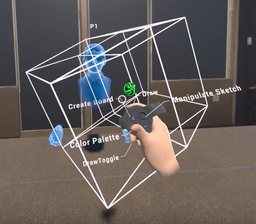
\includegraphics[width=0.2\paperwidth]{presentation.jpg}
    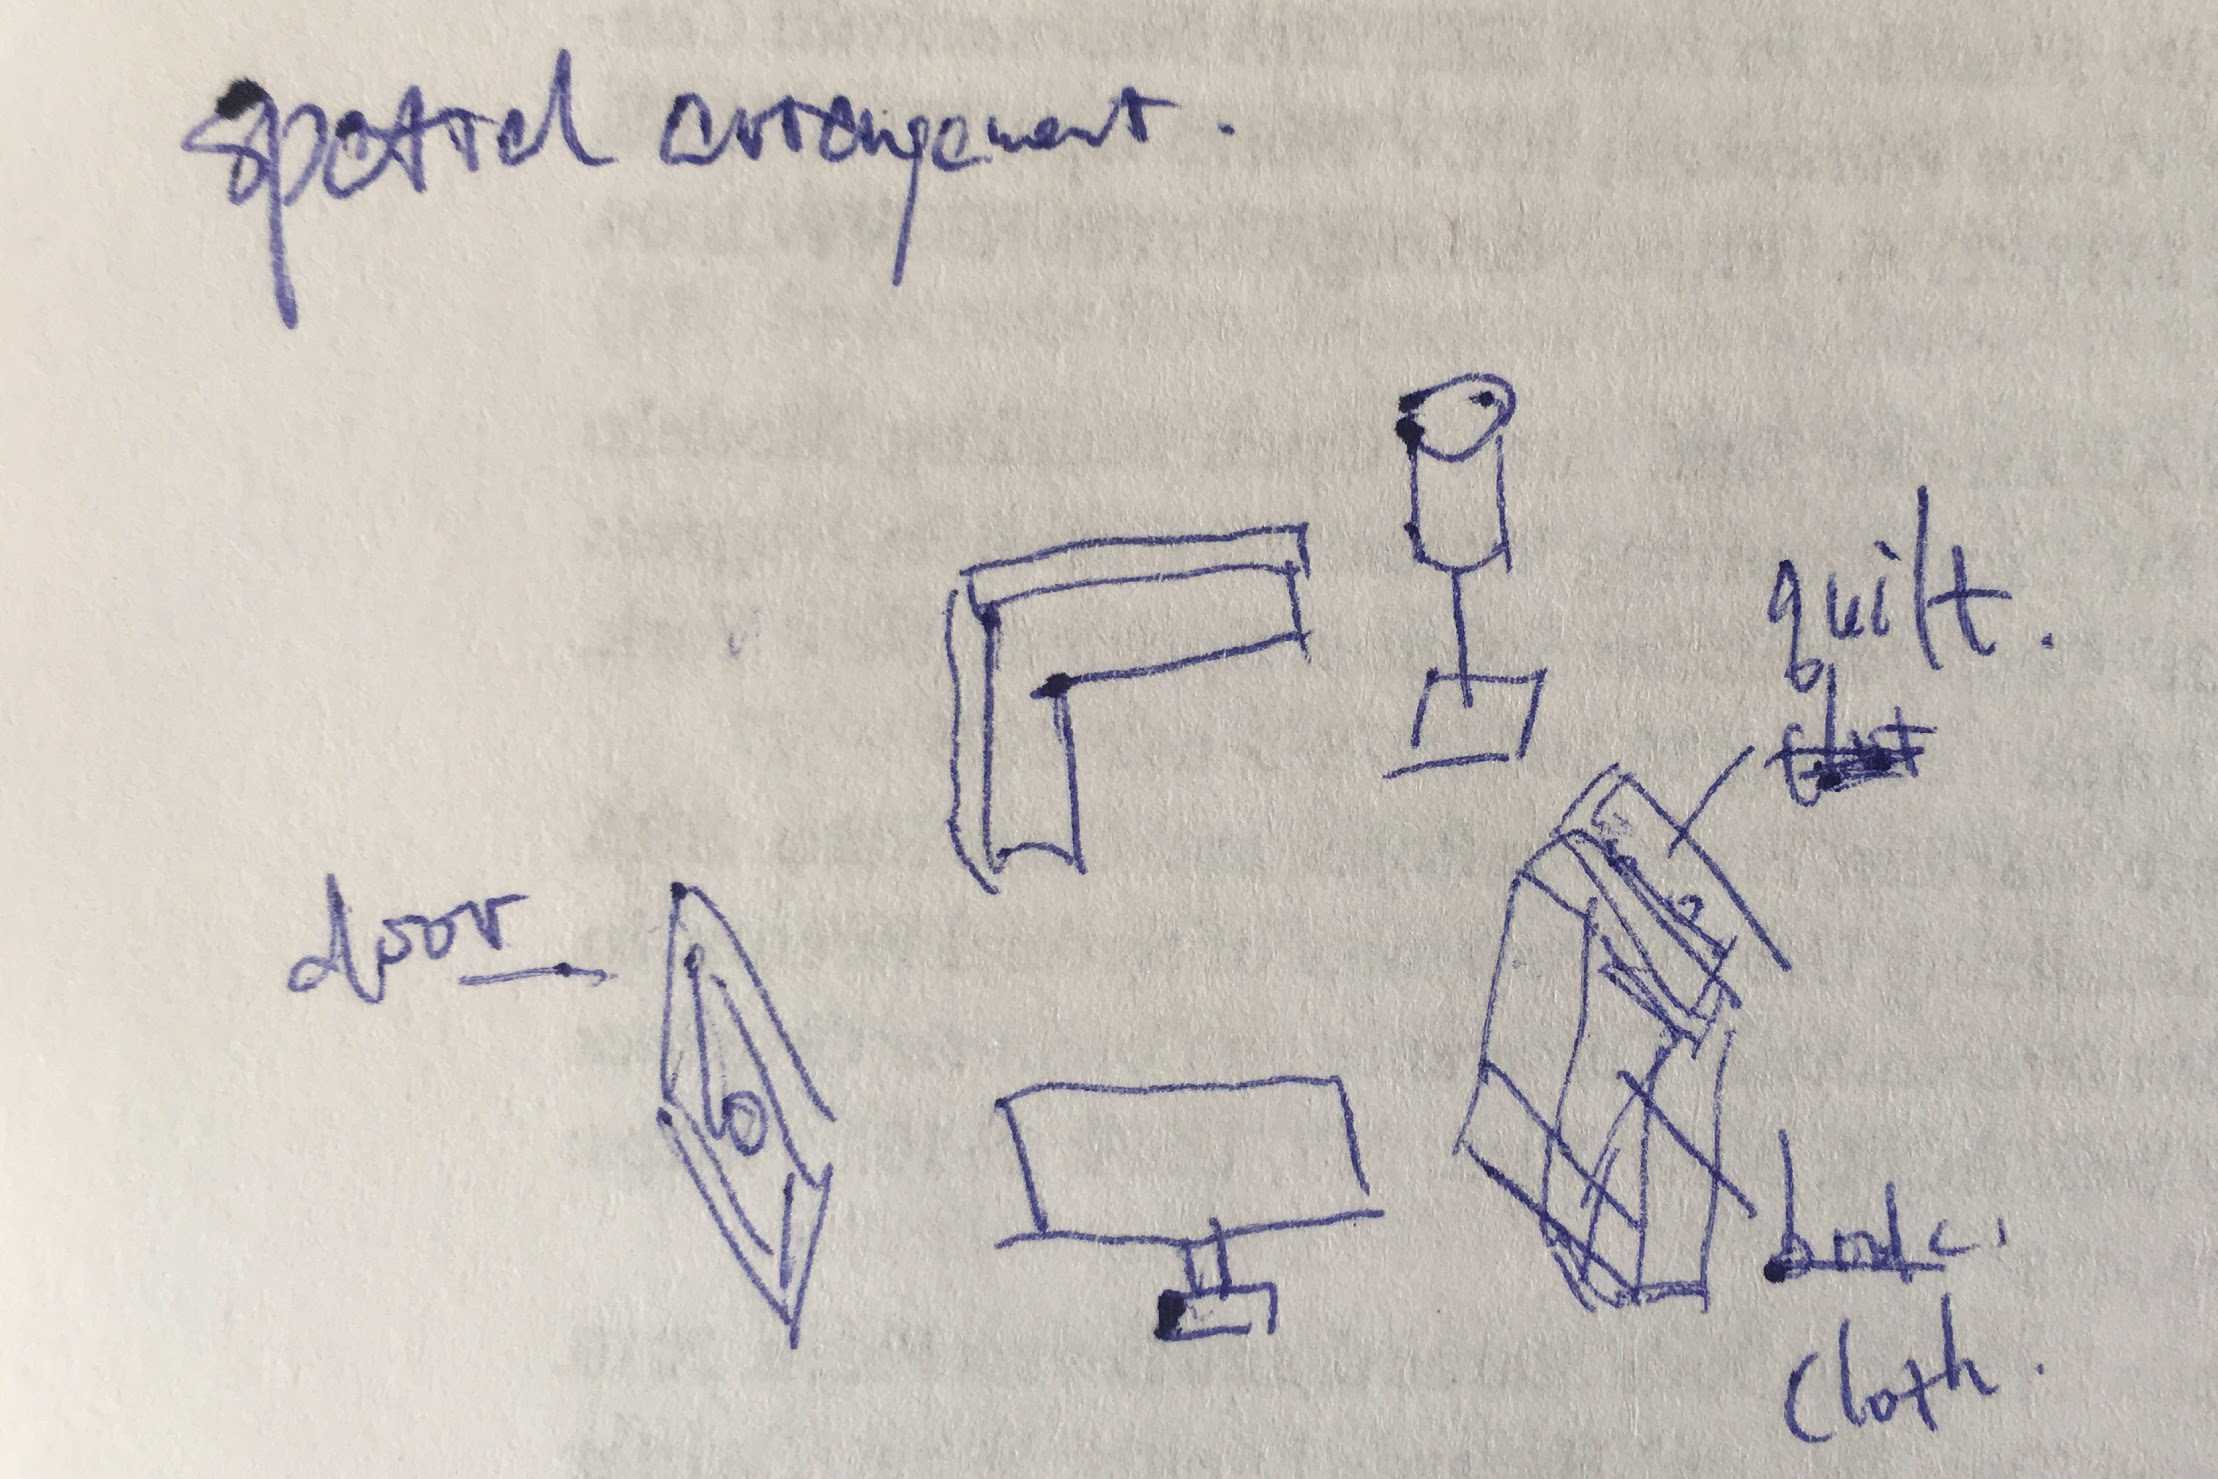
\includegraphics[width=0.2\paperwidth]{spatialarrangement.jpg}
    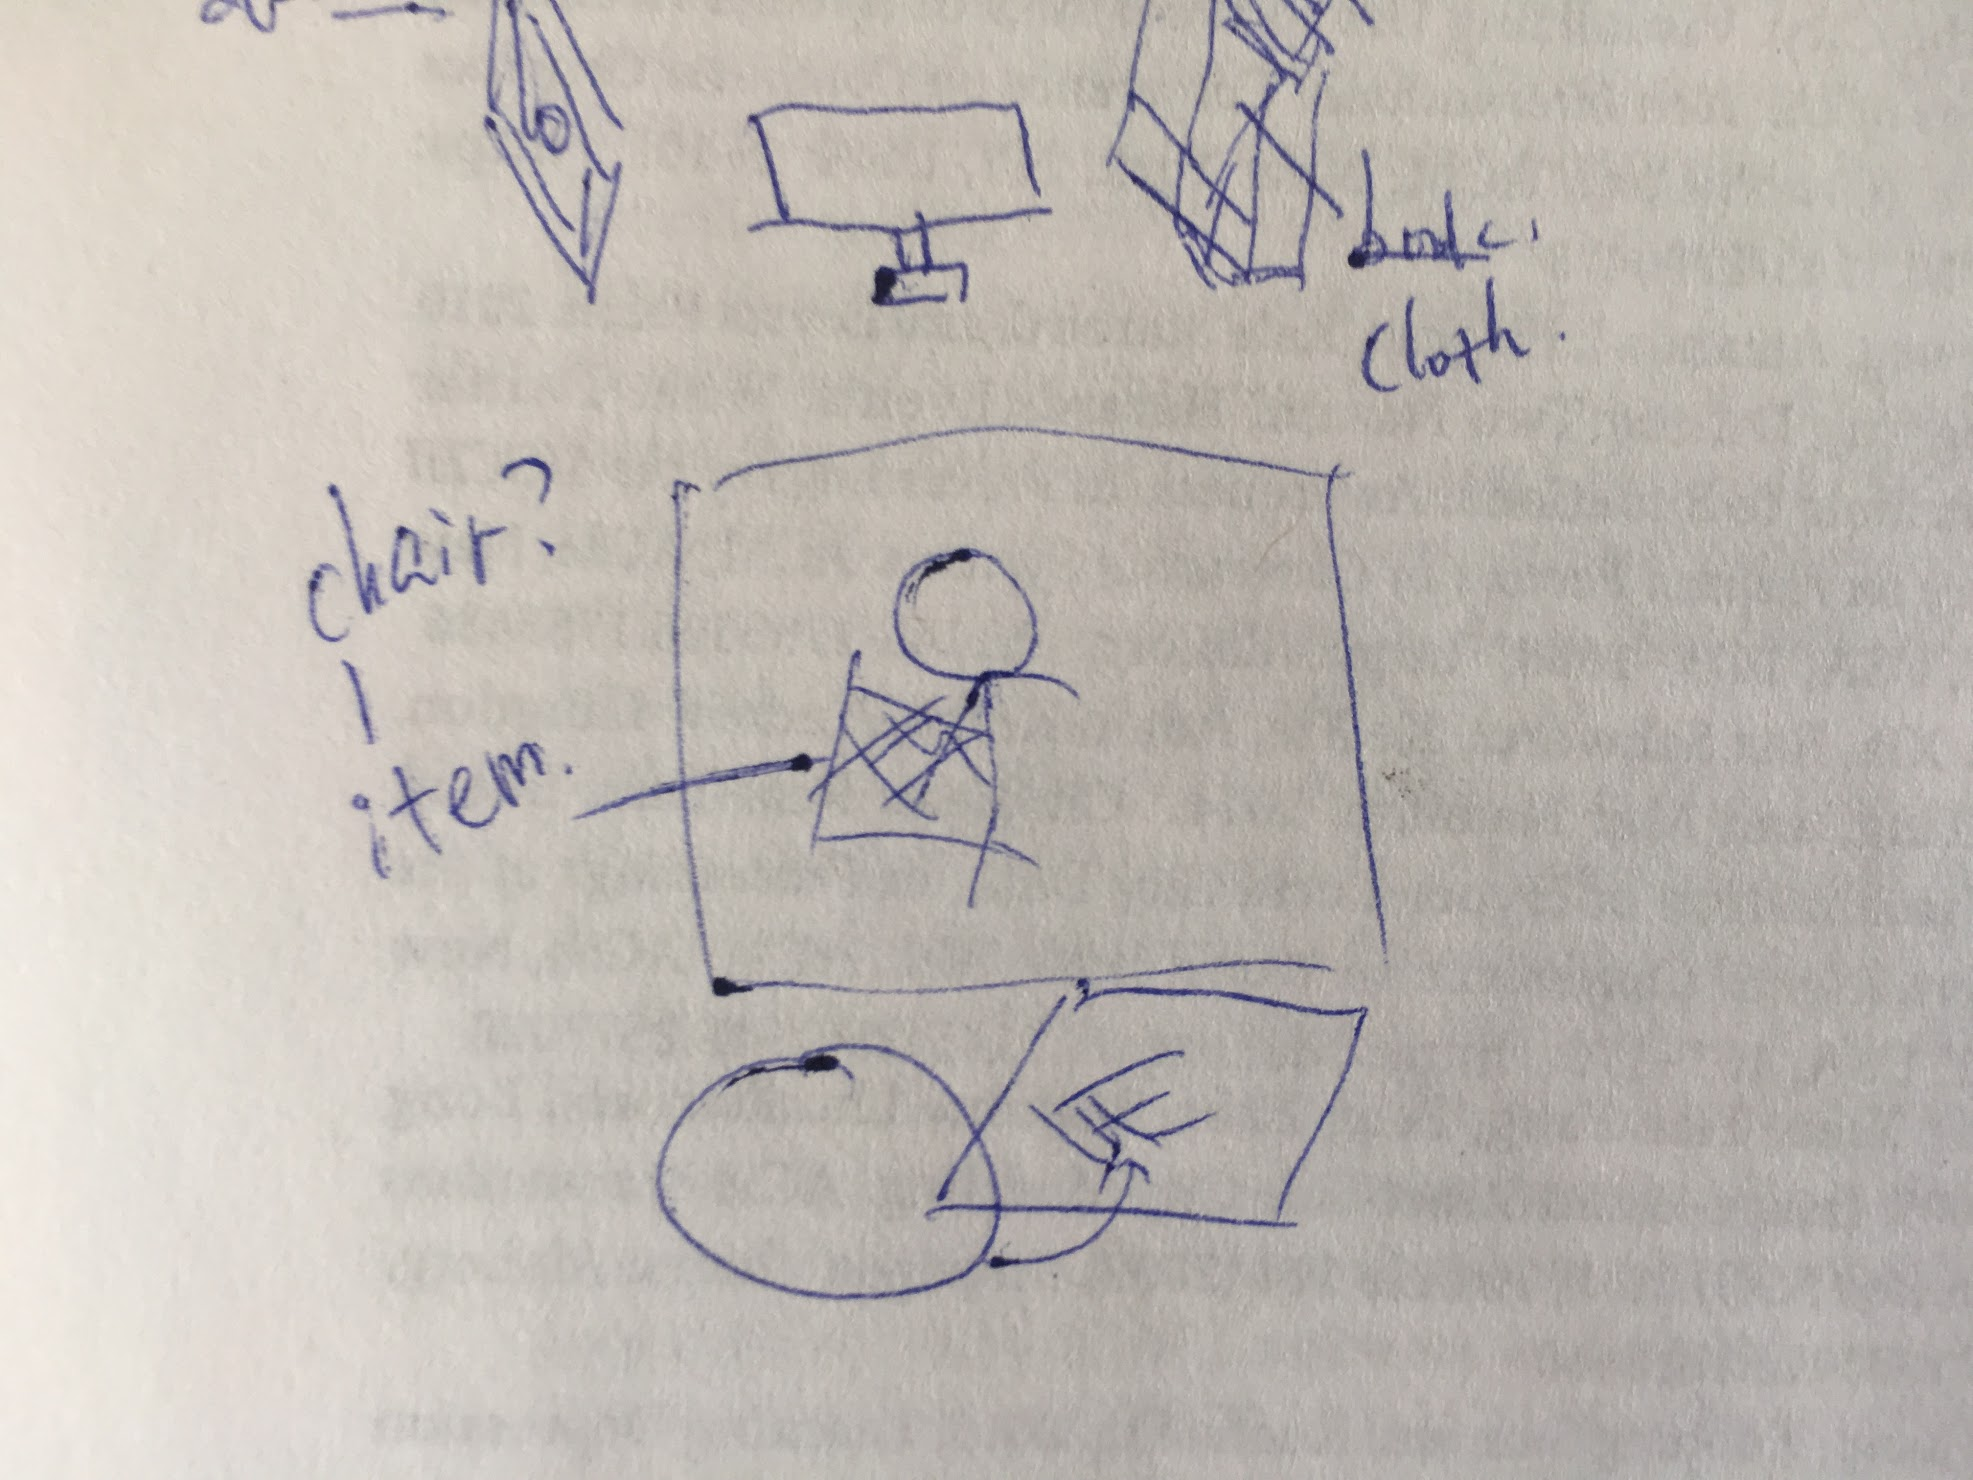
\includegraphics[width=0.2\paperwidth]{itemdesign.jpg}
%\end{subfigure}
\caption{Insert a caption below each figure. Do not alter the
    Caption style.  One-line captions should be centered; multi-line
    should be justified. }
\label{fig:teaser}
} %using an entire image for final version
 
\maketitle

\begin{abstract}
  Despite various collaborative software that supports expressing ideas, people still largely prefer physical notebooks or whiteboards. The reason is that they provide free-form expressions, co-presence of all participants and easy collaboration. However, when working with remote participants, people often choose the convenience of video conferencing, perhaps with screen sharing. We propose CollaboVR, an open-source reconfigurable framework for distributed and co-located multi-user communication in Virtual Reality. We tested CollaboVR with an application that lets participants create freehand drawings and 3D objects, while allowing participants to adjust two key variables: (1) User arrangement (participants adjust the location of their views of other participants) and (2) Input orientation (participants adjust the input to be vertical or horizontal). Preliminary user studies show that CollaboVR is a useful collaborative tool. Users report that some user arrangements and input orientations work best for brainstorming, while others work best for presentation or collaborative refinement of designs.
\end{abstract}


% ACM Classfication

\begin{CCSXML}
<ccs2012>
<concept>
<concept_id>10003120.10003121.10003124.10010866</concept_id>
<concept_desc>Human-centered computing~Virtual reality</concept_desc>
<concept_significance>500</concept_significance>
</concept>
<concept>
<concept_id>10003120.10003121.10003124.10011751</concept_id>
<concept_desc>Human-centered computing~Collaborative interaction</concept_desc>
<concept_significance>500</concept_significance>
</concept>
</ccs2012>
\end{CCSXML}

\ccsdesc[500]{Human-centered computing~Virtual reality}
\ccsdesc[500]{Human-centered computing~Collaborative interaction}

% Author Keywords
\keywords{\plainkeywords}

% Print the classficiation codes
%\printccsdesc
%Please use the 2012 Classifiers and see this link to embed them in the text: \url{https://dl.acm.org/ccs/ccs_flat.cfm}



\section{Introduction}
% VR for workspace and collaboration, however the communication layer still remain the same for most of them
% communication work. Workspace awareness is one important key. -- user arrangement design
% Inspired by taxomony and other tabletop work, we proposed ... a reconfigurable ... to see how mid-air visual aids work and how the two vars affect the experience
% List all the contributions
Virtual Reality (VR) is being explored increasingly, spurred by the availability of high quality consumer headsets in recent years. VR enables rich design spaces in HCI by providing 3D input and immersive experiences. In 1998, an idea, the "Office of the future," was proposed to enable remotely located people to feel as though they were together in a shared office space~\cite{raskar1998office}, via a hybrid of modalities including telepresence, large panoramic displays and manipulation of shared 3D objects. The core idea was that VR had the potential to enhance communication and collaboration among groups of people, as well as Augmented Reality (AR) and projection-based immersive experience. Since then, significant progress has been made in exploring techniques for communication~\cite{ishii1993integration, otsuka2016mmspace}, collaborative works~\cite{kunert2014photoportals,tang2010three}, infrastructure~\cite{maimone2013general, o2011blended, thomas2014muvr} and various modalities~\cite{follmer2013inform, leithinger2014physical, leithinger2015shape, nakagaki2019inforce} for multi-user experiences. However, we found quite a few work are still using 2D audio as the only direct communication method during the collaborative immersive experience~\cite{xia2018spacetime}, let alone some work only provide indirect communication approach such as changing the color of the shared target~\cite{huo2018synchronizar}. In this work, we consider designing a VR communication framework which could be potentially benefited from by collaborative experiences.

% How other ppl contribute to related area, communication/collaboration/co-located and distributed
Quite a few work contributed to improving communication through VR/AR or tabletops for co-located and distributed groups. Observed by Lindemann ~\cite{tversky2003human}, we commonly use gestures or visual aids while speaking to others in daily life. Technically, being aware of these behaviors is part of \textit{workspace awareness}, defined as the up-to-the-moment understanding of other person's interaction with a shared workspace~\cite{li2014interactive}. Providing workspace awareness is widely applied on many works. 
%Prior work tried to improve communication using alternative arrangements of spaces and enhanced digital content for communication. 
One trend is enabling face-to-face interaction during communication through shared display, such as VideoDraw~\cite{tang1990videodraw}, ClearBoard~\cite{ishii1993integration} and FacingBoard~\cite{li2014interactive}. In addition, MMSpace implemented kinetic display avatars so the displays can change self-orientation to realize face-to-face interaction for different participants accordingly~\cite{otsuka2016mmspace}. Besides, traditional setup including white-boards and side-by-side projected displays improved group performance as well~\cite{plaue2009presence}. Another trend is using tabletop tangible devices~\cite{brave1998tangible, kunert2019multi}. 
This setup also provides the co-presence of the other people in the group. Inspired by the previous works, we propose to support different options for user arrangement (how participants adjust the views of other participants) and input orientation (how participants adjust the angle of the input plane).

We propose CollaboVR, an open-source reconfigurable framework for distributed and co-located multi-user communication in VR. The framework includes:
\begin{itemize}
    \item A protocol: connect the portable application to the system. To provide rich and smart visual aids, we choose Chalktalk (an open-source digital presentation and communication language) to support free-hand drawing and 3D objects~\cite{perlin2018chalktalk}. More details will be described later.
    \item A star network: to connect all distributed clients with each other through the server.
    \item Rich interactions on manipulating the drawings: all the visual aids (free-hand drawing or 3D objects) could be further manipulated after being drawn.
    \item Multiple user arrangement: participants can adjust the location of their views of other participants.
    \item Multiple input orientation: participants can adjust the angle of input area.
\end{itemize}

Our main contributions in this papers are:
\begin{enumerate}
    \item Designing and implementing an open-source reconfigurable framework for multi-user communication. The code will be made available \url{masked For Anonymity}.
    \item A system evaluation indicates that CollaboVR is a useful collaborative tool in terms of communication.
    \item Qualitative feedback indicates that different combinations of two key variables (user arrangement and input orientation) work differently for communication in terms of different collaborative purposes.
\end{enumerate}

%\section{Scenario[opt]}

\section{Related Work}
% not smooth
CollaboVR is a framework to assist communication. By definition, communication is an act of expressing and understanding among a group. This is quite similar to \textit{sensemaking}: understanding the meaning~\cite{paul2009understanding}. Sensemaking is a concept widely researched in information visualization area recently. Dervin describes sensemaking as using ideas, emotions and memories to bridge a gap in understanding in group~\cite{dervin1992mind}. Learning how collaborative sensemaking is supported through different design considerations is very inspiring for multi-user communication. In next section, we will introduce collaborative sensemaking approaches first. Second, we will introduce that workspace awareness has positive effects on collaboration and how previous works enhance workspace awareness. Lastly, we will introduce immersive collaboration and communication as well as their gains and limitations.

\subsection{Collaborative Sensemaking}
%introduce the definition of sensemaking somewhere and how we deal with it
Quite a few work have researched sensemaking in different domains in CHI and CSCW area~\cite{albolino2007sensemaking, billman2007medical, landgren2007study,paul2009understanding}. Given that sensemaking involves data analyze~\cite{yi2008understanding}, different designs of 2D displays and digital tabletop are discussed a lot. First, large and shared displays have been shown to benefit sensemaking groups in a number of contexts. Sharodal designed CoSense~\cite{dervin1992mind} with a shared display, conducted an ethnographic study, and examined how collaborative sensemaking can be supported. Moreover, Vogt et al. found that the large display facilitated the paired sensemaking process, allowing teams to spatially arrange information and conduct individual work as needed~\cite{vogt2011co}. Similarly, multiple digital tabletops were used for sensemaking tasks~\cite{isenberg2010exploratory,morris2010wesearch}. Second, personal displays may lead to decreased collaboration in co-located settings ~\cite{chung2013investigating, wallace2009investigating}.

When designing CollaboVR, we take the idea of "multiple" displays, displays with "different" angles, and "personal" display into consideration. That leads to the design of different input orientations and the placement of visual aids.

\subsection{Workspace Awareness}
Workspace awareness is the collection of up-to-the-minute knowledge a person uses to capture another's interaction with the workspace~\cite{gutwin1996workspace}. It includes the awareness of others' locations, activities, and intentions relative to the task and to the space. Maintaining workspace awareness enables participants to work together more effectively~\cite{gutwin1998design, gutwin2002descriptive}. To be more specific, workspace awareness played an important role when dealing with: (1) Simplifying the communication, (2) Taking turns and (3) Action prediction ~\cite{gutwin2002descriptive}. So maintaining and enhancing workspace awareness is beneficial to collaboration. One trend is using see-through displays for distributed collaboration. The idea started with Tang and Minneman who designed VideoDraw~\cite{tang1990videodraw} and VideoWhiteBoard~\cite{tang1991videowhiteboard}. Both approaches are two-user experiences. On each side, a video camera was placed to capture the local user and drawing. A projector was attached to show the remote user and drawing on the top of local display. ClearBoard~\cite{ishii1992clearboard} extended the idea and used digital media. Instead of using projector, the media displayed the video feed of remote user and drawing to keep the workspace awareness. Similarly, KinectArms~\cite{genest2013kinectarms} used tangible tabletop as the media and rendered arm of remote user for mixed presence. Furthermore, Jiannan et al.~\cite{li2014interactive} developed FacingBoard with two-sided transparent displays. Same to ClearBoard, the entire upper-body will be displayed to the other participants so the gaze awareness is supported. To keep the gaze interaction, FacingBoard reversed the graphics on the display. However, some column-sensitive content such as text and map became incorrect. To solve this problem, FacingBoard selectively flipped the column-sensitive content individually and adjusted the position of the content. However, when people were pinpointing a specific sub-area within the content, the gaze and the place being pinpointed were inconsistent to all the users. In our system, we proposed different user arrangements to enhance workspace awareness. We also provide the similar face-to-face experience. Differently, we manipulate user's locations to keep the gaze awareness rather than flipping the content and we support more than two people. This will be described in detail later.

// todo
MetaSpace did full body tracking for distributed users to create a better sense of presence~\cite{sra2015metaspace}. 

\subsection{Immersive Collaboration and Communication}
% we need more and more because reviews were complaining the amount
% think about the trend
Much work has been done in collaborative applications in VR/MR.
Some focused on multi-user gaming experiences. SynchronizAR designed a registration algorithm for mobile AR so the participants could join the co-located experience and not need to take extra steps to ensure good-quality positional tracking~\cite{huo2018synchronizar}.
Some focused on developing telepresence and bridging the gap between physical world and virtual world. InForce created a set of novel interaction techniques including haptic feedback for distributed collaboration ~\cite{nakagaki2019inforce}.
Holoportation demonstrated 3D reconstructions of an entire space including people reconstruction~\cite{orts2016holoportation}.
Immersive Group-to-Group Telepresence ~\cite{beck2013immersive}
Some designed a collaborative tool for productive work like editing and modeling. SpaceTime focused on improving the experience for two experts collaborating on design work together~\cite{xia2018spacetime}. 
Some put more effort on object manipulation and navigation.
T(ether) is a spatially-aware display system for co-located collaborative manipulation and animation of objects ~\cite{lakatos2014t}. Trackable markers on pads and digital gloves allow participants to use gestures to manipulate objects in space.
Andre et al. designed an application to support object manipulation tasks and scene navigation from different views ~\cite{kunert2019multi}.
Some developed the distributed system for remote assistance.
Virtual Replicas for Remote Assistance is a remote collaboration system, allowing a remote expert to guide local users to assemble machine parts by using virtual replicas~\cite{oda2015virtual}.
Others like Geollery~\cite{du2019geollery, du2016social} created an interactive mixed reality (MR) social media platform.

For collaborative purposes like social network and telepresence, the engagement and sense of being there is the most important. In those scenarios, the communication is not the focus. While for collaborative purposes such as productive work, game, assistance or object manipulation, which require complicated and specific operation and information transfer during the collaboration, the communication performance becomes more important. We want to build a reconfigurable framework to fit different purposes of collaboration.

Then we take a look at the trending of communication with immersive environments.
% fill with old submission and go through chi+cscw+uist for recent 5 years.
Some proposed asymmetrical communication. ShareVR enables communication between an HMD user and a non-HMD user~\cite{gugenheimer2017sharevr}. By using floor projection and mobile displays to visualize the virtual world, the non-HMD user is able to interact with the HMD user and become part of the VR experience. Mutual human actuation~\cite{cheng2017mutual} run pairs of users at the same time and have them provide human actuation to each other. The communication between the pair is through shared interactive props.

Interacting with digital content in a shared space is common too. Three's Company~\cite{tang2010three} explored collaborative activities over connected digital tabletops which support a shared sense of presence among people and artifacts associated with the task. 
Dyadic projected spatial augmented reality 
TwinSpace supports deep interconnectivity and flexible mappings between virtual and physical spaces~\cite{reilly2010twinspace}.
Your Place and Mine explored three ways of mapping two differently sized
physical spaces to shared virtual spaces to understand how social presence, togetherness, and movement are influenced~\cite{sra2018}.
Tan et al. built a face-to-face presentation system for remote audiences ~\cite{gazeAwareness}.
Tele-Board~\cite{gumienny2011tele} designed a groupware system specialized in creative working modes using traditional whiteboard and sticky notes in digital form for distributed users.
Hrvoje Benko et al. proposed a unique spatial AR system that enables two users to interact with a shared virtual scene and each other in a
face to face arrangement~\cite{benko2014dyadic}. 
We found out quite a few work focused on two-user or pair communication. Our work proposed a solution to scale the amount of the participants. In addition, we noticed much work experiment the face-to-face setup with shared display or round table for communication. We propose two variance: user arrangement and input orientation to investigate their advantages and limitation.

%In daily life while speaking to others, we commonly use gestures or visual aids~\cite{tversky2003human} to help present ideas, either subconsciously or purposefully. Visual aids can be drawn on paper, a whiteboard\cite{cherubini2007let}, or a screen via desktop sharing in video conferences. A key task for collaborators is visually, physically, and cognitively following the content being drawn and the people who are speaking with. They need a clear view of the content under discussion and need to be aware of other collaborators' presence when communicating~\cite{ishii1992clearboard}. They should also understand and be able to reason about what is being shown and said. 
%According to Regenbrecht et al.~\cite{regenbrecht2015mutual}, facial interaction like eye contact and mutual gaze has always been recognized as an important requirement for effective visual communications. That suggests it is helpful during communication to look at the person who is talking or at least be aware of the person's location. 
%Oftentimes, participants in a group discussion also need to move around physically to follow the content and each other. In addition, following and presenting content requires the ability to express ideas clearly as well as a fair understanding of the ideas. This may become particularly challenging in discussions revolving around, for example, the placement and design of 3D objects, which cannot easily be visualized using traditional 2D communication media (paper, whiteboard, and so on).

\section{CollaboVR Overview}
In this section, we present an overview of CollaboVR's system architecture. CollaboVR consists of a protocol which serialize the display data from an application and then de-serialize and render them into graphics. Currently we test CollaboVR with application Chalktalk~\cite{perlin2018chalktalk}. Chalktalk is an open-source digital presentation and communication language. It allows a presenter to create and interact with animated digital sketches on a blackboard-like interface. There are some other smart sketch-based online software such as Autodraw~\cite{Autodraw}, sketch2code~\cite{Sketch2code} and Miro~\cite{Miro} can assist drawing. We chose to use Chalktalk because it is an open-source platform. We can easily define the dataflow between the application and CollaboVR. That means if the API of input and output of the application is accessible, CollaboVR can be easily adapted to use multiple applications as the content provider.

\begin{figure*}[ht!]
 \centering
 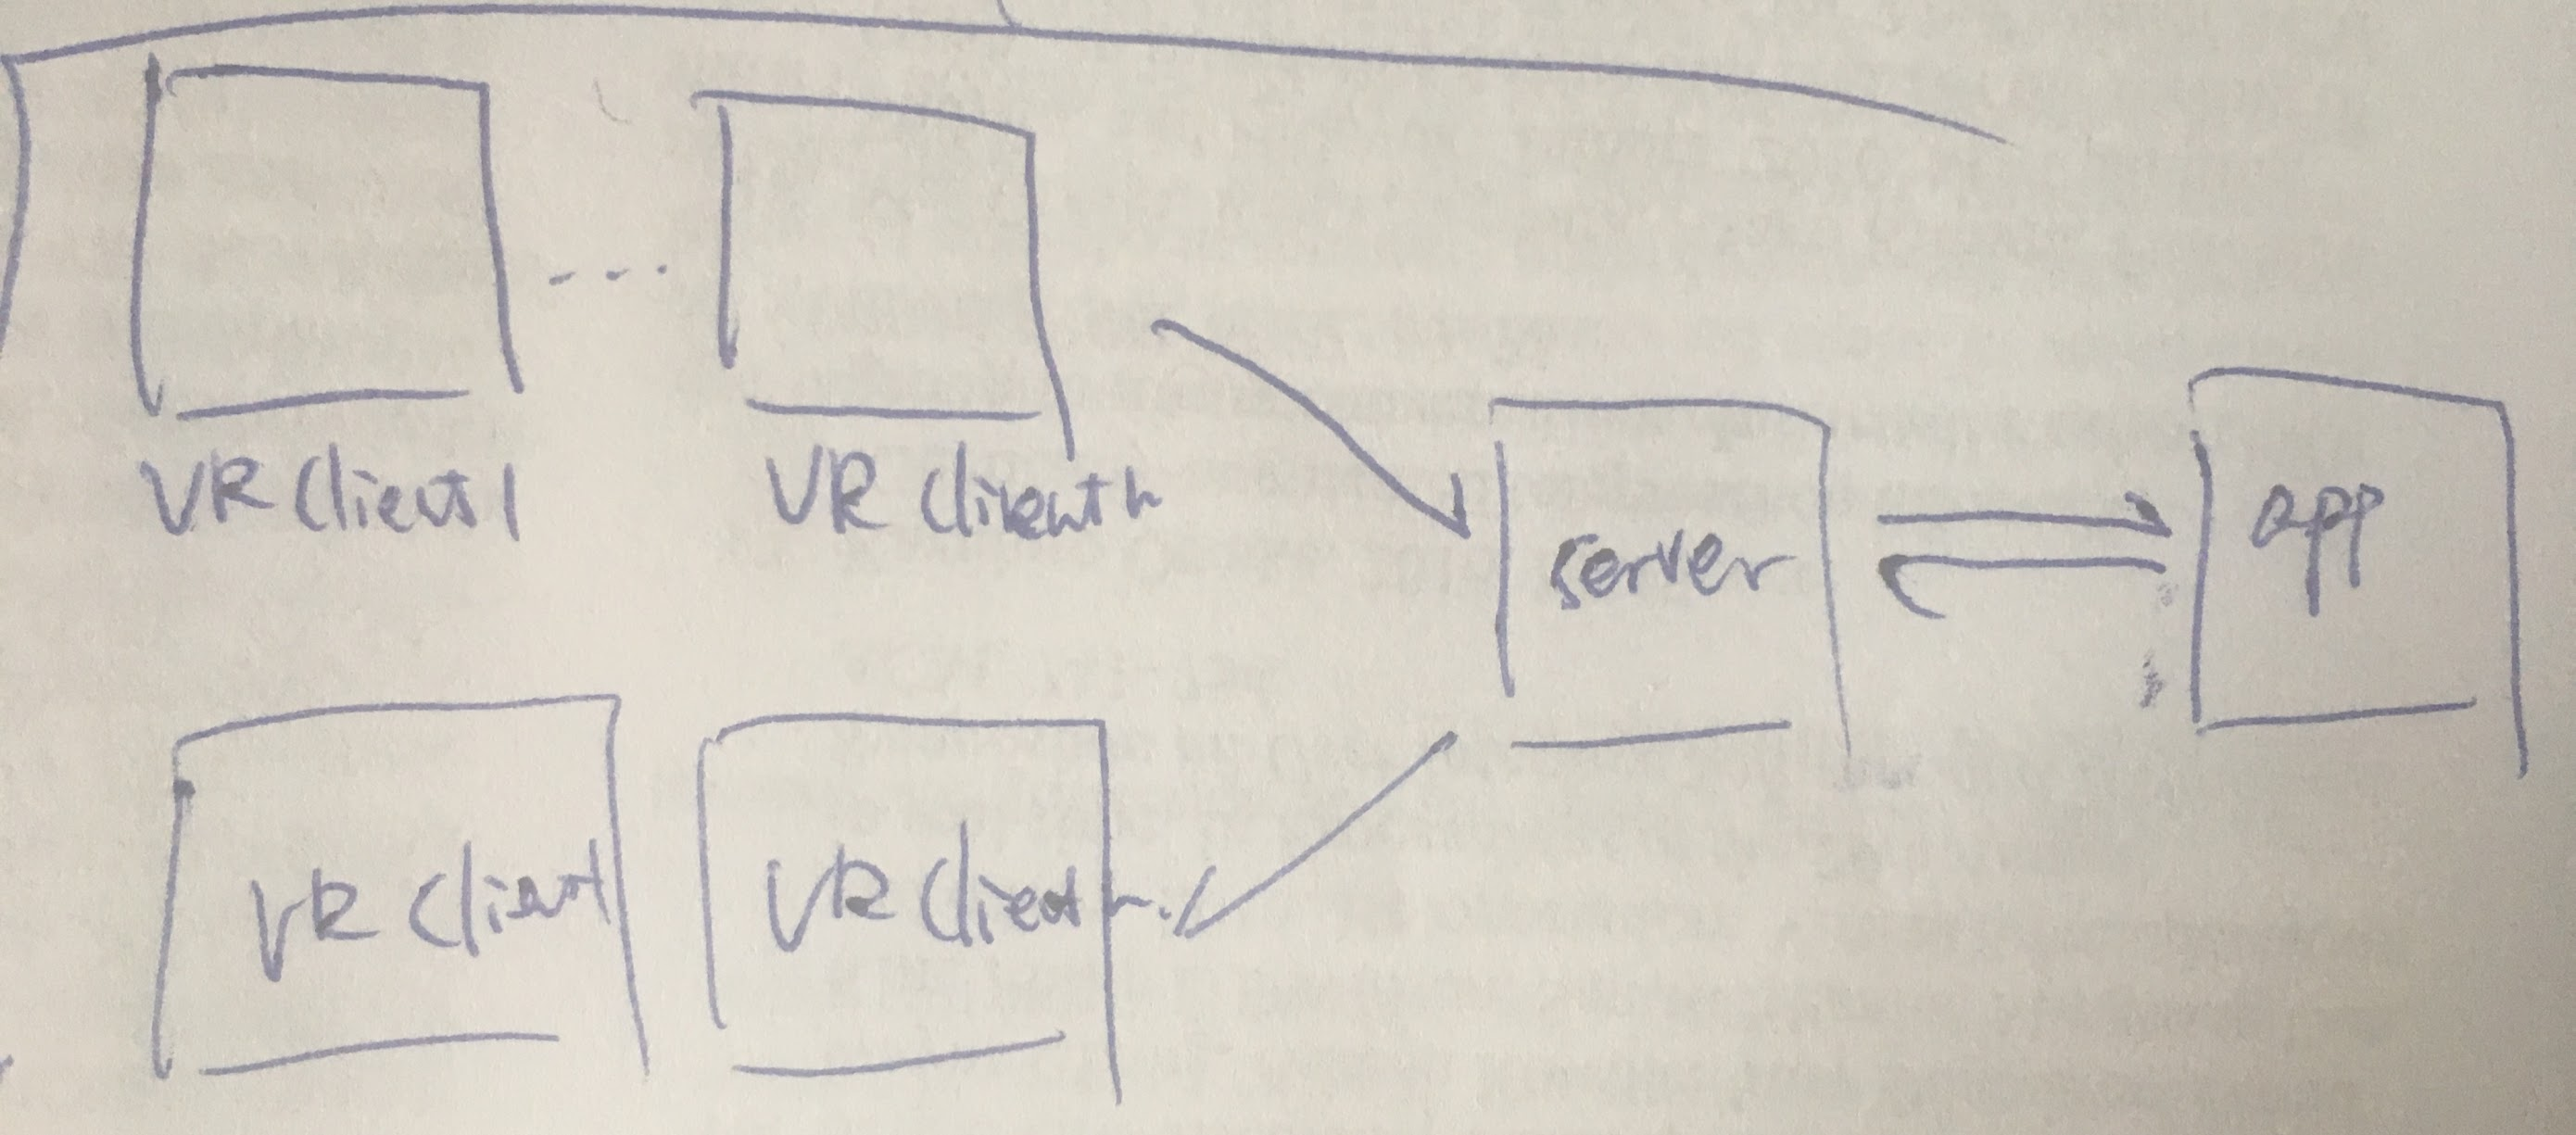
\includegraphics[width=1.75\columnwidth]{workflow}
 \caption{The workflow of CollaboVR.
 %Chalktalk's content, \textit{sketch} is composed of graphical elements such as point data. 
 // TODO
 %1) \textit{Sketch} data are serialized on the Chalktalk client side every frame and 2) sent as a data array to the Chalktalk server, 3) to the Holojam relay, and then 4) to all Unity clients, where 5) the data are rendered on content board(s). 6) MR user input is sent back through the pipeline to the Chalktalk client and 7) translated into HTML canvas mouse events. 8) Avatar synchronization data are also sent between clients using the Holojam relay.
 }~\label{fig:workflow}
\end{figure*}

CollaboVR consists of a star network. The network is written in Node.js and C\#. It synchronizes data across devices and supports custom data formats. For CollaboVR, we have two kinds of information: rendering data and user data. In terms of rendering data, we first pass the user input from each client to the server, then the server transmits the user input with the user identifier to the application, next the server receives the serialized display data from the application, finally the server broadcast the display data to each client for rendering. In terms of user data, we currently don't do any process on it so we directly broadcast the user avatar and audio data to each client.

CollaboVR consists of rich interactions on manipulating the drawings. After the clients receive and render the display data from the application, the display data is considered as interactive object in 3D world. We provide manipulation on these objects for users to express their ideas easily. The manipulation includes: duplication, transformation(rotating, scaling and translation), deletion, and colorization.

To deploy CollaboVR, it only requires a VR device running Unity for each client, a server machine running the Node.js (if a VR client needs to be run on a Windows machine, the server code could run on one of the client machines) and a router (optional) which ensures the low latency for data transmission. If a router is not available for setup, all the clients can talk to server through IP address over the Internet. 

% talking about architecture with figures
% Explain the entire pipeline and Chalktalk

Figure ~\ref{fig:workflow} presents the workflow of CollaboVR per frame. First, figure~\ref{fig:workflow}(a) and figure~\ref{fig:workflow}(b) show the third-person perspective view of the VR client before data synchronization. The user in figure~\ref{fig:workflow}(a) is drawing a dinosaur to show what is his or her favorite animal. The user in figure~\ref{fig:workflow}(b) is waiting. Then the data including both users' identifier, avatar information, audio and the drawing input information will be serialized and send to the server. As figure~\ref{fig:workflow}(c) shows, different data will be processed with different label such as \verb|AVATAR_JOIN|, \verb|STYLUS|, \verb|SELECT_OBJ|, \verb|MOVE_OBJ|. The server is behaved as a state-less machine. So the server send the drawing input related data to application API and broadcast avatar related code to all the clients. Later, the application received the drawing input data from the server as figure~\ref{fig:workflow}(d) shows. The application (Chalktalk) will process the input and turn the drawing into 3D objects. We can see that the free-hand drawing dinosaur becomes a 3D dinosaur with pre-designed animation. Our protocol serialized \verb|DisplayData| from application (Chalktalk) and send to the server. The server broadcast \verb|DisplayData| to all the clients. Finally, all the VR clients can see the interactive 3D objects and each other as figure~\ref{fig:workflow}(e) and figure~\ref{fig:workflow}(f) show.

\section{Design Space}
We propose two variables in the design space of CollaboVR: user arrangement and input orientation. Emphasized by the previous work on workspace awareness that maintaining and enhancing workspace awareness enable participants to work together more effectively. We add a dimension that users can change their views of other participants. In other words, they can manipulate the arrangement of other users. 

Inspired by the previous work on collaborative sensemaking, we notice that multiple and shard large displays are good for collaborative work in terms of 2D information. CollaboVR is an immersive 3D graphics world. Instead of "display", we pre-placed multiple "interactive board" in the virtual environment. That means, if the z coordinate of the content is 0, the connect will be placed on the interactive board. If the content has positive or negative z coordinate, user will see that the content is not stitch to the interactive board. The relative coordinate system is the center of the corresponding interactive board. We add a dimension that users can change the input orientation of the interactive board in axis x (from 0$^{\circ}$ to 90$^{\circ}$). Considering the learning curve for the users, we simply provide two edge options: vertical (0$^{\circ}$) and horizontal (90$^{\circ}$) interactive board.

\subsection{User Arrangement}
Currently, we provide two user arrangements: (1) default and (2) mirrored. Default user arrangement means that the virtual environment of each user will be overlapped directly. As figure~\ref{fig:userarrangement} shows, figure~\ref{fig:userarrangement}(a) and figure~\ref{fig:userarrangement}(b) are two top-down view for each client. The green rectangle shows their available tracking area roughly. The blue rectangles show the interactive boards. Figure~\ref{fig:userarrangement}(c) shows the default user arrangement. The clients will see other participants in their original position. For mirrored user arrangement, all the other users' location will be flipped to the other side of the interactive board. See figure~\ref{fig:userarrangement}(d), user2 is in mirrored user arrangement, and user1 is flipped to the other side of the left interactive board because user1 is looking at that board. Spot A is the same content that both users are looking at. After the flipping operation, the gaze direction of user1 and user2 are maintained. Different from FacingBoard~\cite{li2014interactive}, the content is not mirror reversed so the content is still correct to the viewer. In this user arrangement, the users can see each other for better workspace awareness. Figure~\ref{fig:userarrangement}(f) shows how we process multiple users in this setup. Each user will be flipped based on their looking direction.

\begin{figure}[t!]
 \centering
 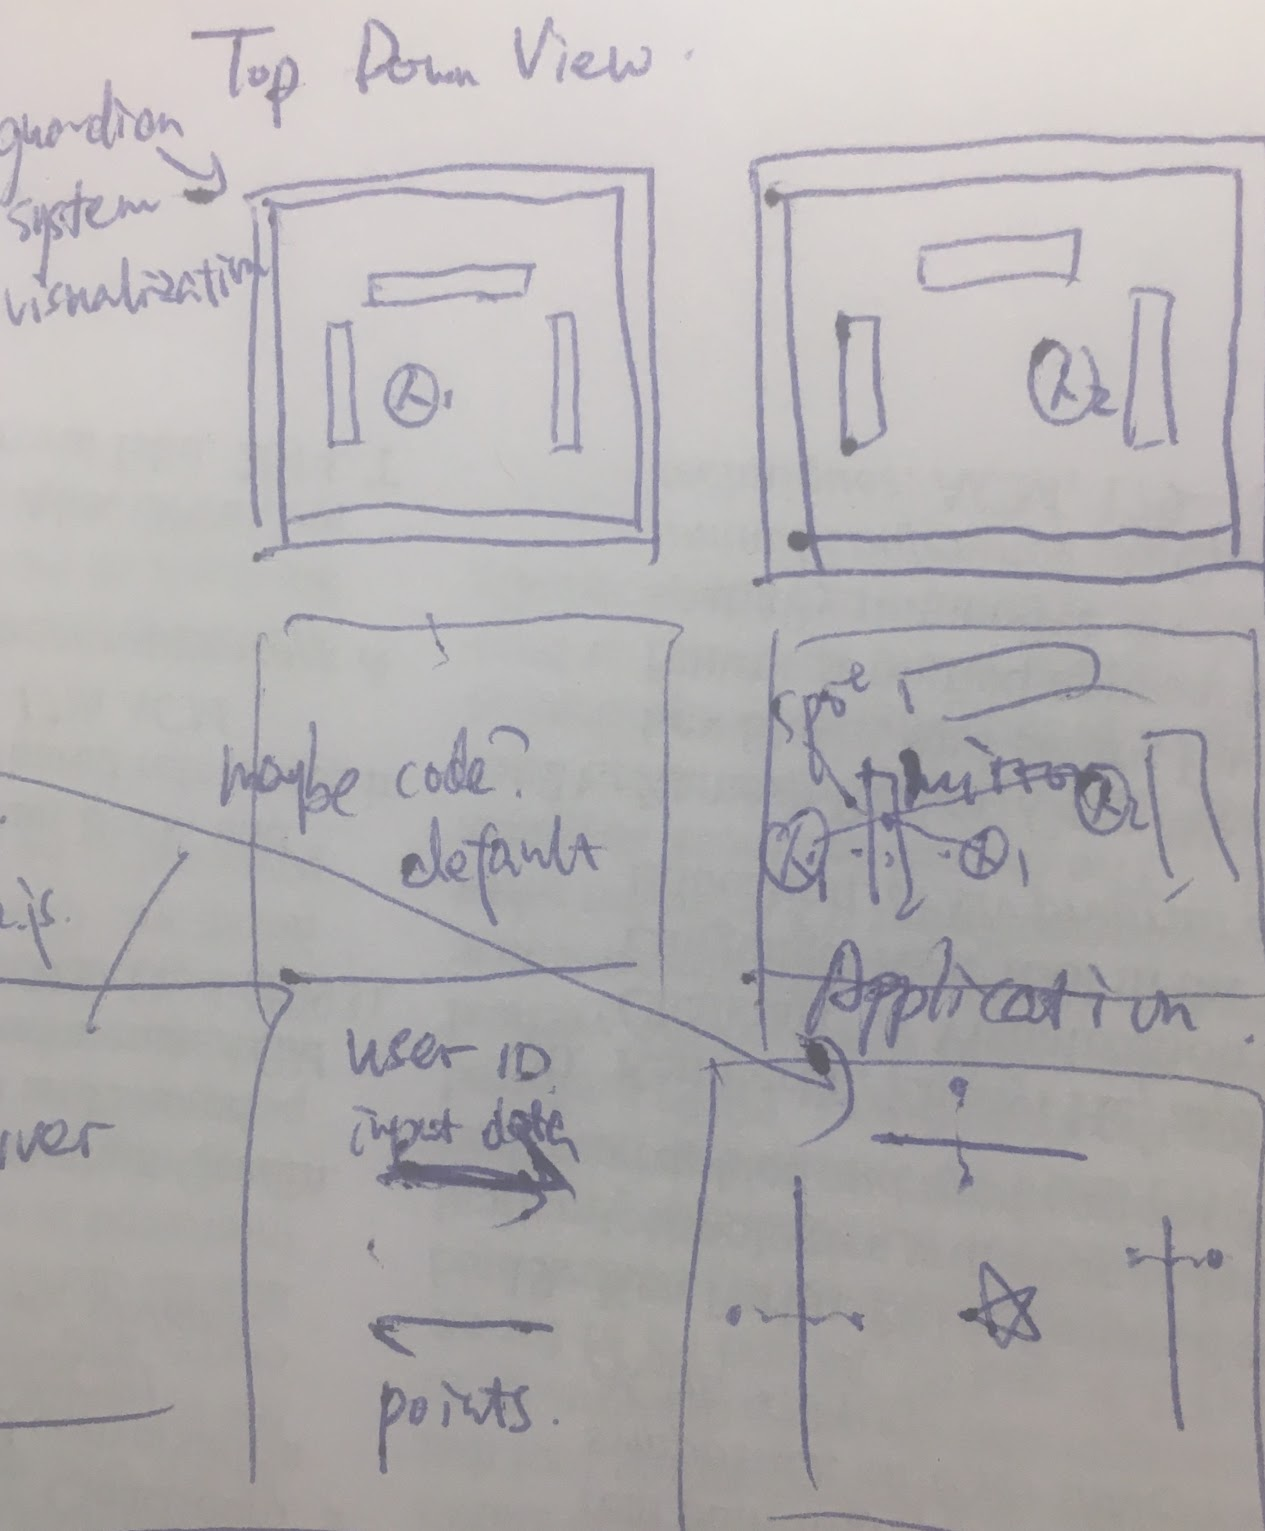
\includegraphics[width=0.9\columnwidth]{userarrangement.jpg}
 \caption{Design space: user arrangement.
 }~\label{fig:userarrangement}
\end{figure}

\subsection{Input Orientation}
CollaboVR enables the user to adjust the interactive board for input: vertical or horizontal board. By default, the interactive board is vertical as a large display, but in 3D. As figure~\ref{fig:inputorientation}(a) shows, user's experience is close to writing on a white-board. When user turns on the horizontal interactive board, it is close to writing on a tablet or desk, as figure~\ref{fig:inputorientation}(b) shows. For other users who are not writing, the content will be rendered real-timely on the vertical board. By doing this we avoid the situation that the content is not readable for all the users around a table. Considering the reach distance when writing on a horizontal plane is different from on a vertical plane, we adjust the scale of the horizontal board. When user is writing on the horizontal board, he or she is free to look at the personal horizontal board or the shared vertical board. To enhance the awareness of where the user is writing on, we render the projection point of user's controller as a 3D cursor.

\begin{figure}[b!]
 \centering
 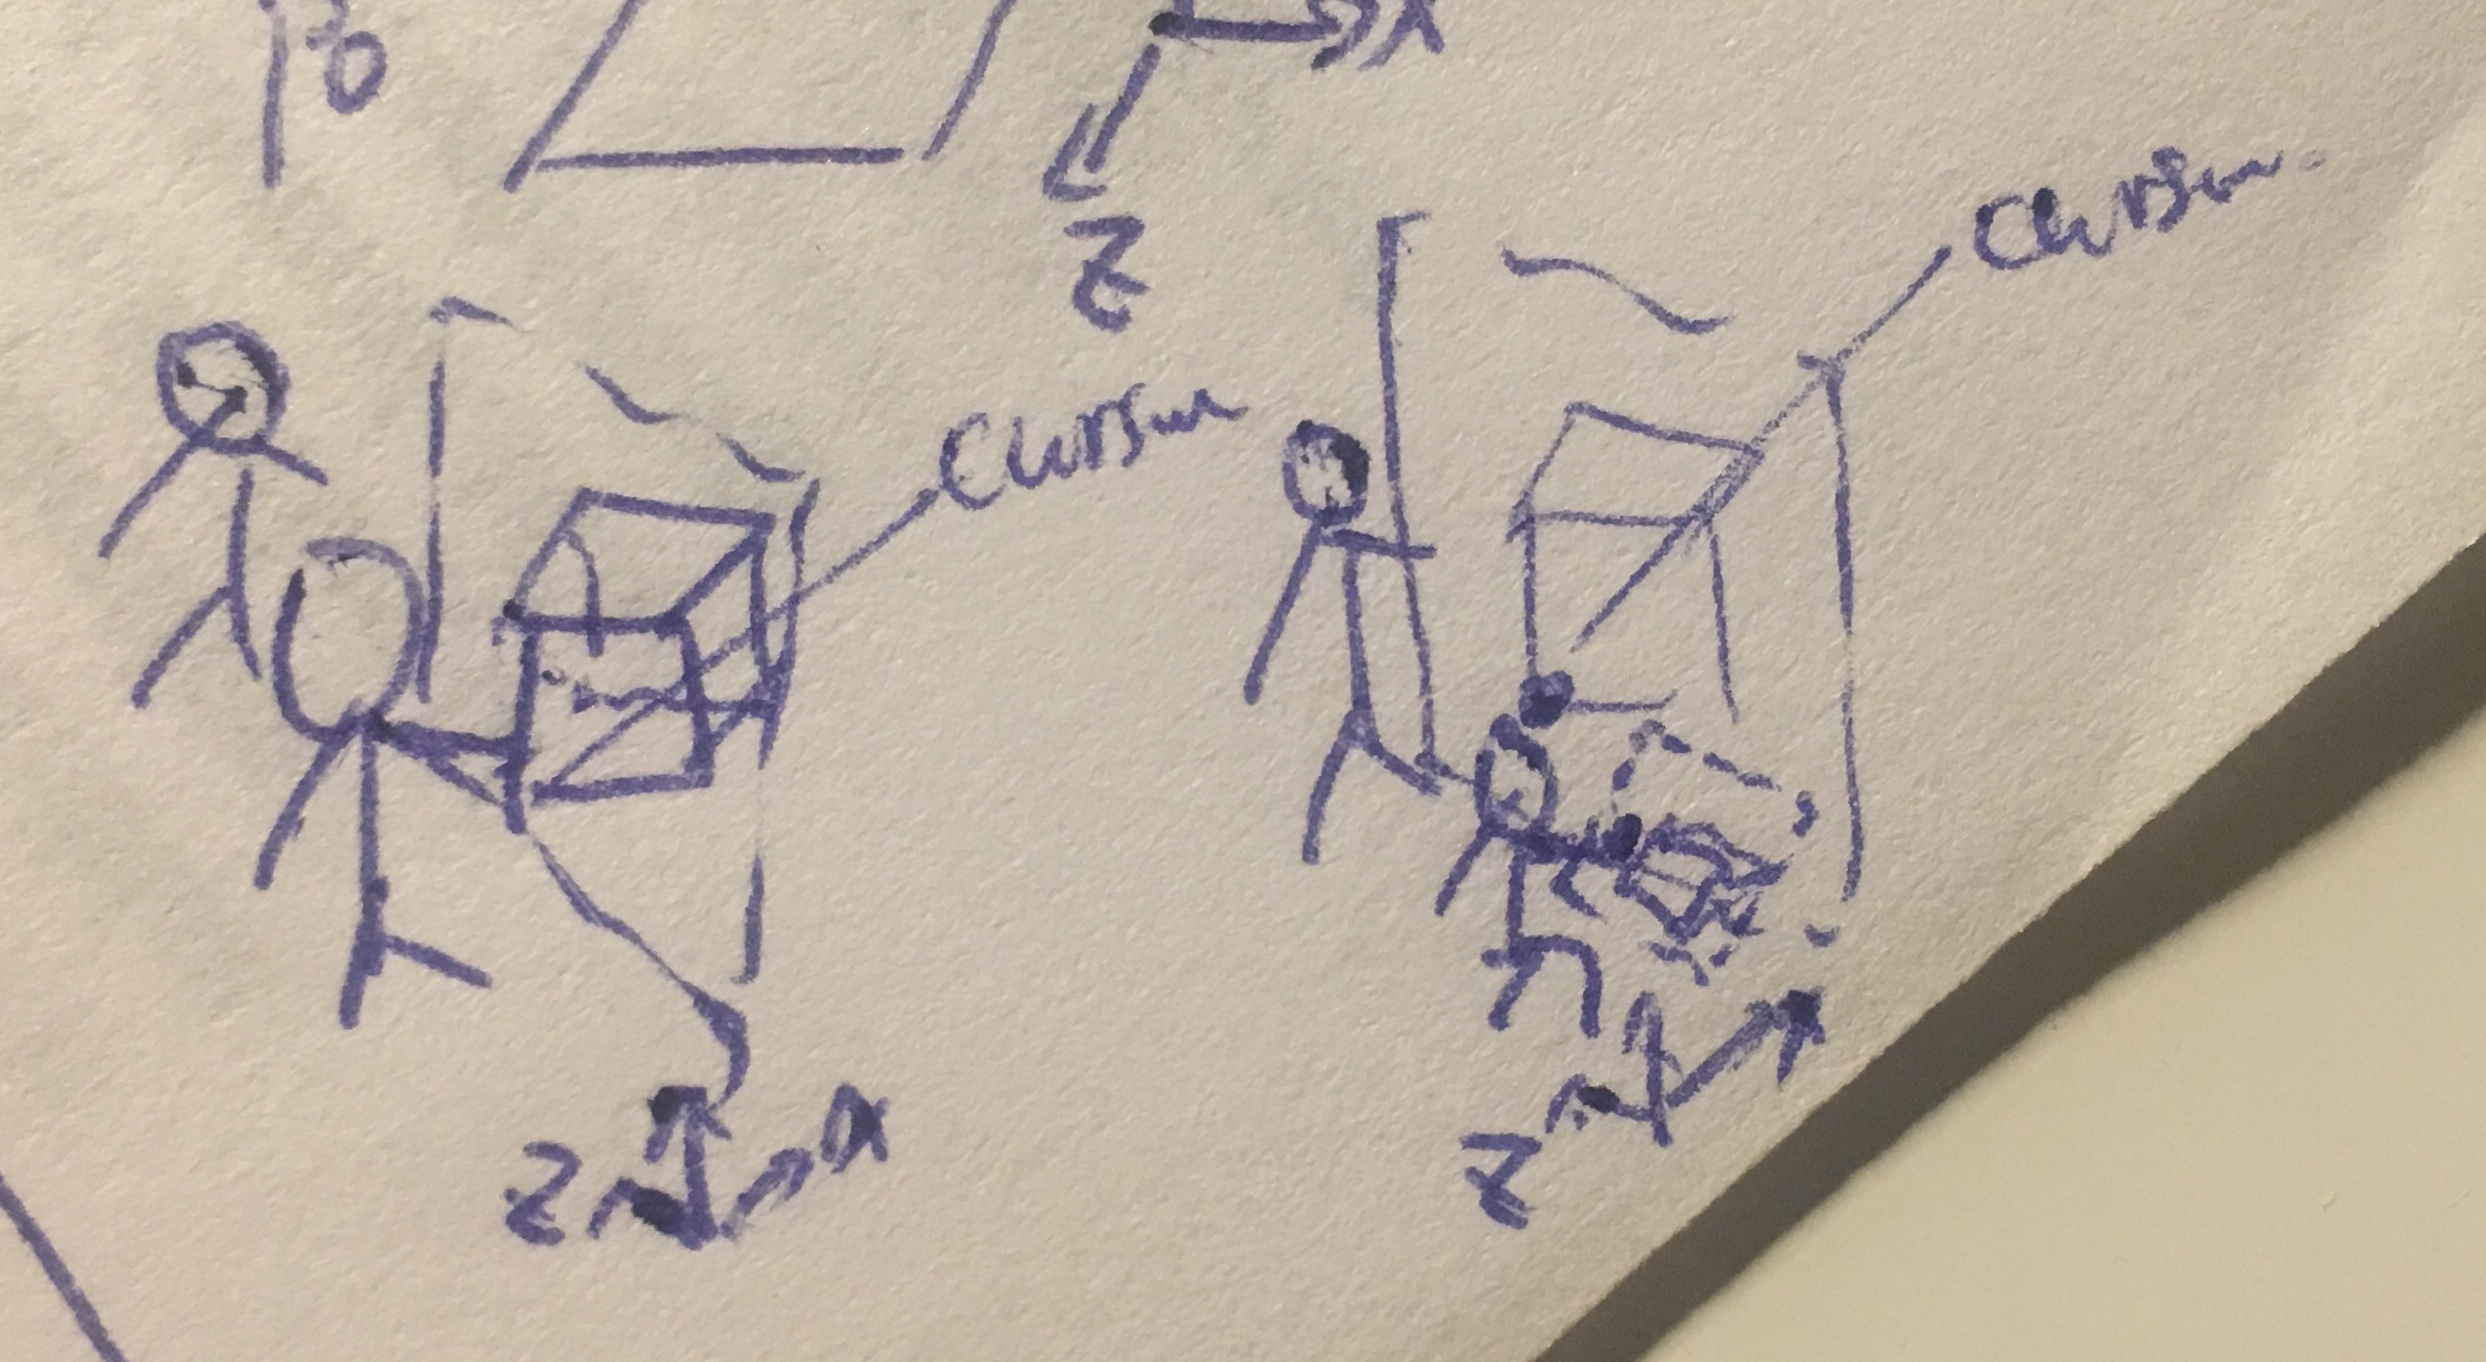
\includegraphics[width=0.9\columnwidth]{inputorientation.jpg}
 \caption{Design space: input orientation.
 }~\label{fig:inputorientation}
\end{figure}

\section{System Implementation}
To build CollaboVR, we implement a network framework and a flexible protocol, a calibration approach for co-located users, user interface for drawing manipulation and other functionalities.

\subsection{Network and Protocol}
The network is a star network using UDP. The reason we chose UDP is that we value low-latency more than the accuracy. The server-side code is written in Node.js and the client code is written in Node.js and Unity C\#. We defined \textit{synchronizable object}: an object needs to synchronized each frame for the client who registered it. Each synchronizable object has a label and data stream. The label is a unique identifier for client to register. The data stream includes the frequency of sending this object and the real-time data. We provide two kinds of frequency in the system: one-time and per frame. One-time synchronizable object is actually a command. It doesn't happen for each frame and not need to be synchronized for each frame. For command object, we use two-way handshaking. The client sends the object to the server, the server returns an object including acknowledgement back to the client, then the client de-registers the object with this label. Per frame synchronizable object could be the current avatar representation, the audio data or the display data from the application. We design a protocol to wrap all the display data. The data protocol includes information of all the rendered points by encoding the attributes such as position, width and color. Each client de-serialize the data from the server and render the points as lines and meshes.

\subsection{Calibration for Co-located Scenarios}
CollaboVR is working for both co-located and distributed scenarois. For distributed users, we simply overlap their virtual environments because they don't have any spatial relationship. For co-located users, we need to calibrate all the users so they are all in the same coordinate system. The key idea for calibration is that different clients should have a shared proxy. For example, all the co-located users can see the same image in that environment. Vuforia~\cite{Vuforia} is widely used for image recognition and tracking. Similarly, a shared map is helpful too~\cite{Hololens}. Here we use Vive Pro as the co-located device. The shared proxy is the Vive base station. Each machine running Vive can retrieve the transformation information of the base station. Because each machine has their own coordinate systems, we will have the same mount of the position and rotation of base station. We pre-chose one base station as the proxy based on the unique serial number. Then we use the first client which connected to the server as the reference node. All the following clients will apply the inverse matrix between the base station of reference node and their own base station to their VR environment. See figure~\ref{fig:vivepro}, user1 is drawing a physics model. The left image shows the first-player perspective view from user2 and the right image shows a front view of the environment.

\begin{figure}[tb!]
 \centering
 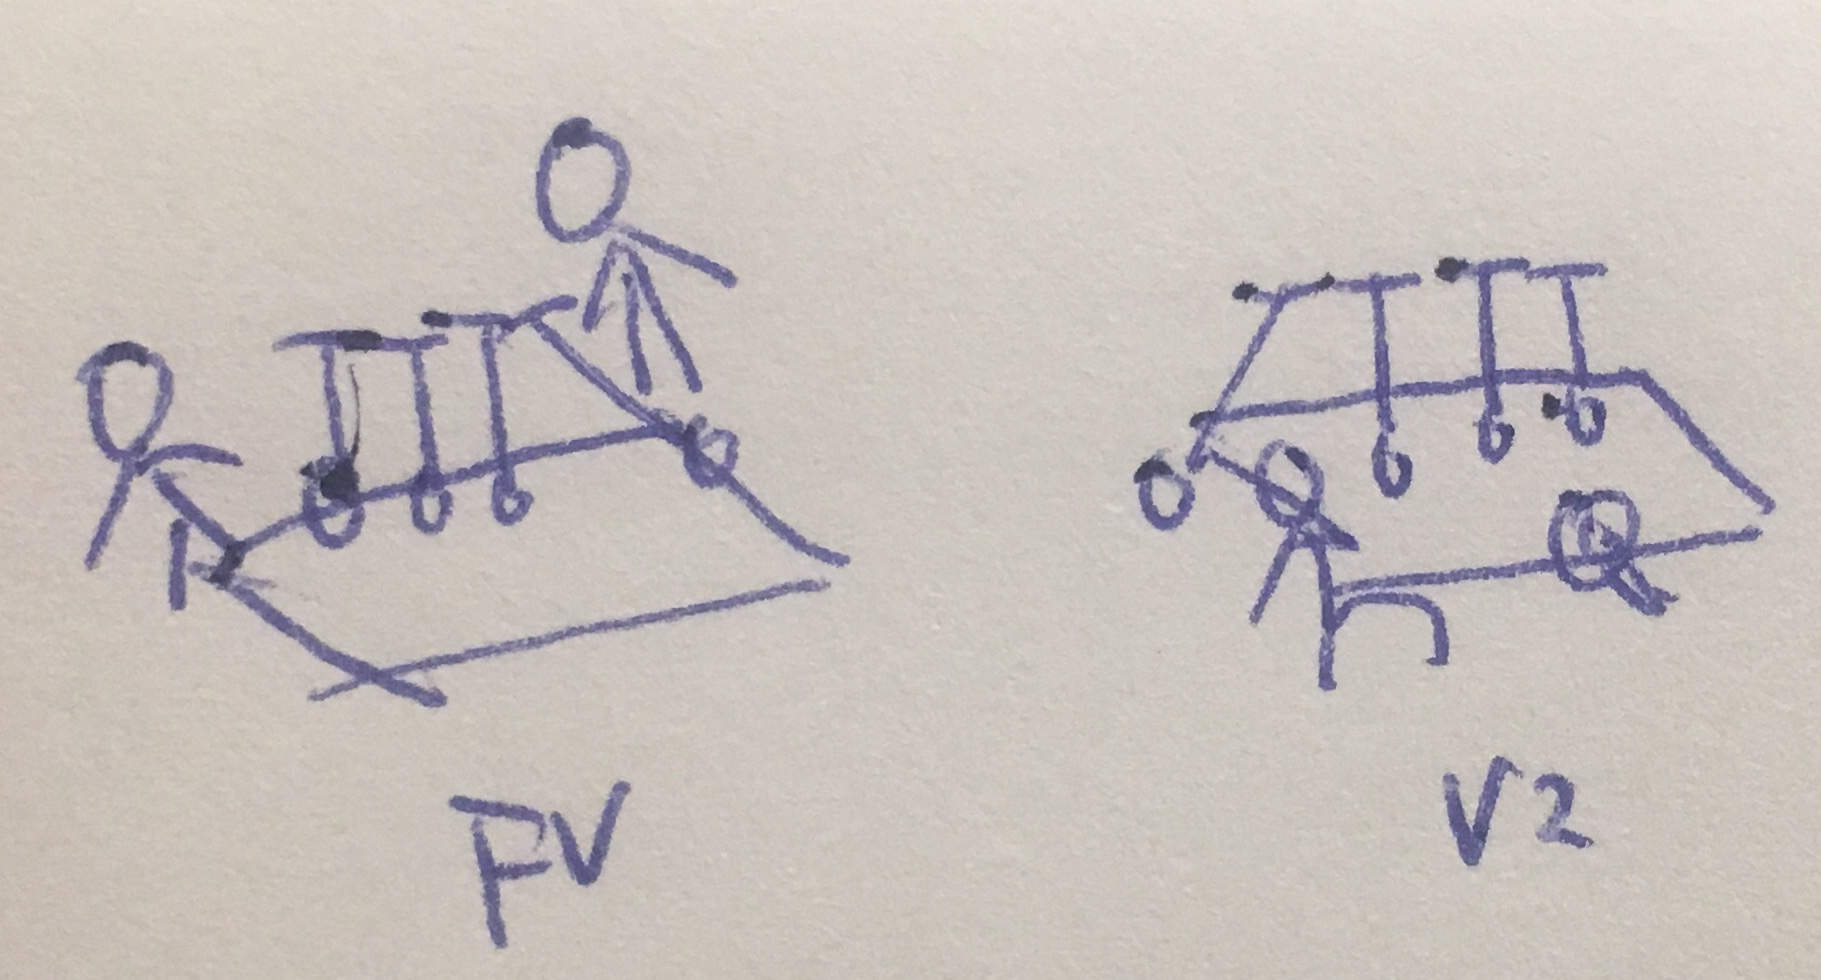
\includegraphics[width=0.9\columnwidth]{vivepro.jpg}
 \caption{Calibration results for co-located users.
 }~\label{fig:vivepro}
\end{figure}

\subsection{Drawing Manipulation}
CollaboVR includes a user interface for users to manipulate the objects after drawing. We provide the functionality of duplication, transforming, deletion and colorizing. To achieve this, we design a pie menu triggered by the controller. Here is the workflow for manipulation: first, we place the controller hovering over the drawing of interest; second, press the thumbstick of the dominate controller; then, the pie menu shows up as figure~\ref{fig:userinterface}; Move the thumbstick to select the specific menu; Apply corresponding movement in terms of the command and release the thumbstick. If the menu is deletion, the operation applies immediately after release. If the menu is transformation, user needs to move the controller to complete rotation, scaling and translation. If the menu is copy, the duplicated object will be placed at the position where the user releases thumbstick. In addition, we enable colorization through another button. User can drag the color from the color palette to any drawing like world builder\footnote{\url{https://www.youtube.com/watch?v=FheQe8rflWQ}}. Colorization is triggered by button one as figure~\ref{fig:userinterface} shows. 

\begin{figure}[tb!]
 \centering
 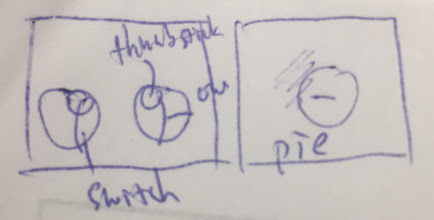
\includegraphics[width=0.9\columnwidth]{userinterface.jpg}
 \caption{User interface for drawing manipulation.
 }~\label{fig:userinterface}
\end{figure}

\subsection{Other}
Considering the system is working identical to left-hand users and right-hand users, button two is designed to switch the commands of two controllers (see figure~\ref{fig:userinterface}). Considering the user's view might be blocked by other users' avatar, we implement spectator mode. User can see the view from different users in the lower right corner. To encourage all the users work on the task together, we implement a permission strategy. There is only one user we can draw at one time. Once the user who is drawing release the permission, other users can grab the permission to draw. Figure~\ref{fig:userinterface} shows the permission indicator.

\section{Use Cases}
CollaboVR is designed as a reconfigurable framework for users to communicate in VR. Here we envision the potential user cases for CollaboVR.

\subsubsection{Daily Life Schedule and Brainstorming}
CollaboVR could be used for daily life schedule as figure~\ref{fig:teaser}(a) shows. With default user arrangement and input orientation, the experience is close to white-board writing. CollaboVR enables free-hand drawing, so users can write and draw their plans and coordinate with friends. Shapes and colors are useful while scheduling. When they have different ideas, user can easily duplicate the current drawing onto another interactive board to express new branches.

\subsubsection{Presentation}
CollaboVR could be used for presentation figure~\ref{fig:teaser}(b) shows. By enabling the mirrored user arrangement and the default input orientation, the presenter and the audience will be placed on two sides of the content. It is easy for the presenter to know where is the audience's focus and useful for the audience to follow the presenter's gesture and content at the same time.

\subsubsection{Spatial Arrangement}
CollaboVR can help with spatial arrangement especially for 3D scenarios. Imaging the user just moves in to a new apartment and needs to discuss the placement of the furniture with roommate. As figure~\ref{fig:teaser}(c) shows, user can draw furniture with the combinations of primitive shapes and place them directly at the place they prefer. The spatial arrangement is difficult to be described clearly through words and gestures. And it often requires multiple views when using drawings.

\subsubsection{Item Design}
CollaboVR can help with collaborative design. By enabling the mirrored user arrangement and horizontal input orientation, user can draw their ideas in detail with friends. The experience is close to drawing on a digital tablet with a pen. Other users can explain their opinions while pointing at the area of interest.

\section{User Study: System Evaluation}

In this study, we evaluated the interaction cycle, design variables and prototype implementation of CollaboVR. We were interested in how participants use the system. During the study, we collected primarily qualitative feedback to gain insight into the experience of using the system.

\subsection{Tasks and Procedure}
Participants were grouped by four. Each group was first given an introduction to the user study and gave consent for video recording. Then they were given a 10 minute lecture through a large monitor on how to use application: Chalktalk. We described how to do freehand drawing and how to create pre-defined 3D objects.
Then for 10 minutes participants were given a live demo on how to use CollaboVR. One experimenter put on the headset and described how to use each controller button and the functionality in the system, including getting permission to draw, manipulating drawings and objects in 3D and other functionalities.
After that, each participant was moved to separate rooms. They learned how to use CollaboVR individually until all of them were able to conduct drawing and manipulation. Then they went to the shared virtual environment for design tasks. 

\subsubsection{Living room design}
All the groups were asked to experience three 10-minute sessions. 
Each session has different combinations for user arrangement and input orientation: condition1 is default user arrangement and input orientation, condition2 is mirrored user arrangement and default input orientation, condition3 is default user arrangement and horizontal input orientation.
We counterbalanced the order of the conditions for each group using Latin Square. For each session, the participants were asked to design a living room containing only three items: one table, one chair and one couch. 
Each participant picked one item and wrote down their designs for the item and the layout of the three items. Then they use CollaboVR to express their original ideas and reach an agreement for the living room design. After each session, they wrote down their final decisions for the design of the living room. The writing will be used for further analysis.
We provided three items for the group (four people) so they needed to resolve conflicts and come up with a final decision for the design of living room.

\subsubsection{Semi-structured interview}
Upon completion of all the sessions, we presented users with a set of statements and asked them to rate how much they agreed with each of them on a 7-point Likert scale. We then went into a semi-structured interview asking about their experience, trying to gain insight into the usability of the system.

\subsection{Participants}
We recruited a total of 12 participants (5 females and 1 left-handed; age range: 20 - 30, $M=23.58$, $SD=3.45$) via campus email lists and word-of-mouth. None of the participants had been involved with this project before. Participants have various VR experience (Rating scale, 1 less experience to 7 a lot of experience, $M=4.08$, $SD=1.83$).

\subsection{Apparatus}
CollaboVR is implemented in Unity on Windows desktops with Nvidia GTX 1080 cards. We used Oculus Rift CV1 with two Oculus Touch controllers, which we paired with one of four computers during the experiments. We connected the four computers to the router through Ethernet cables.

\subsection{Data Collection and Analysis}
The study mainly focused on the system usability and qualitative feedback from the survey and interview. In addition, we conducted one-way analysis of variance (ANOVA) statistical tests to examine the differences between different user arrangement and input orientation on task performance. The task performance is defined as the details of the living room design for each session. We analyzed the writing by calculating the amount of the details such as color, shape, texture and layout. Our null hypothesis is that across different user arrangements and input orientations, there is no difference in task performance. We predict that (1) the mirrored user arrangement foster higher performance and (2) the horizontal input orientation leads to lower performance. Questionnaire data that related to usability of user arrangement and input orientation were analyzed using repeated measures analysis of variance (RM-ANOVA). The level of significance was set at $p<0.05$.

\subsection{Results and Discussion} 
\begin{figure}[tb!]
 \centering
 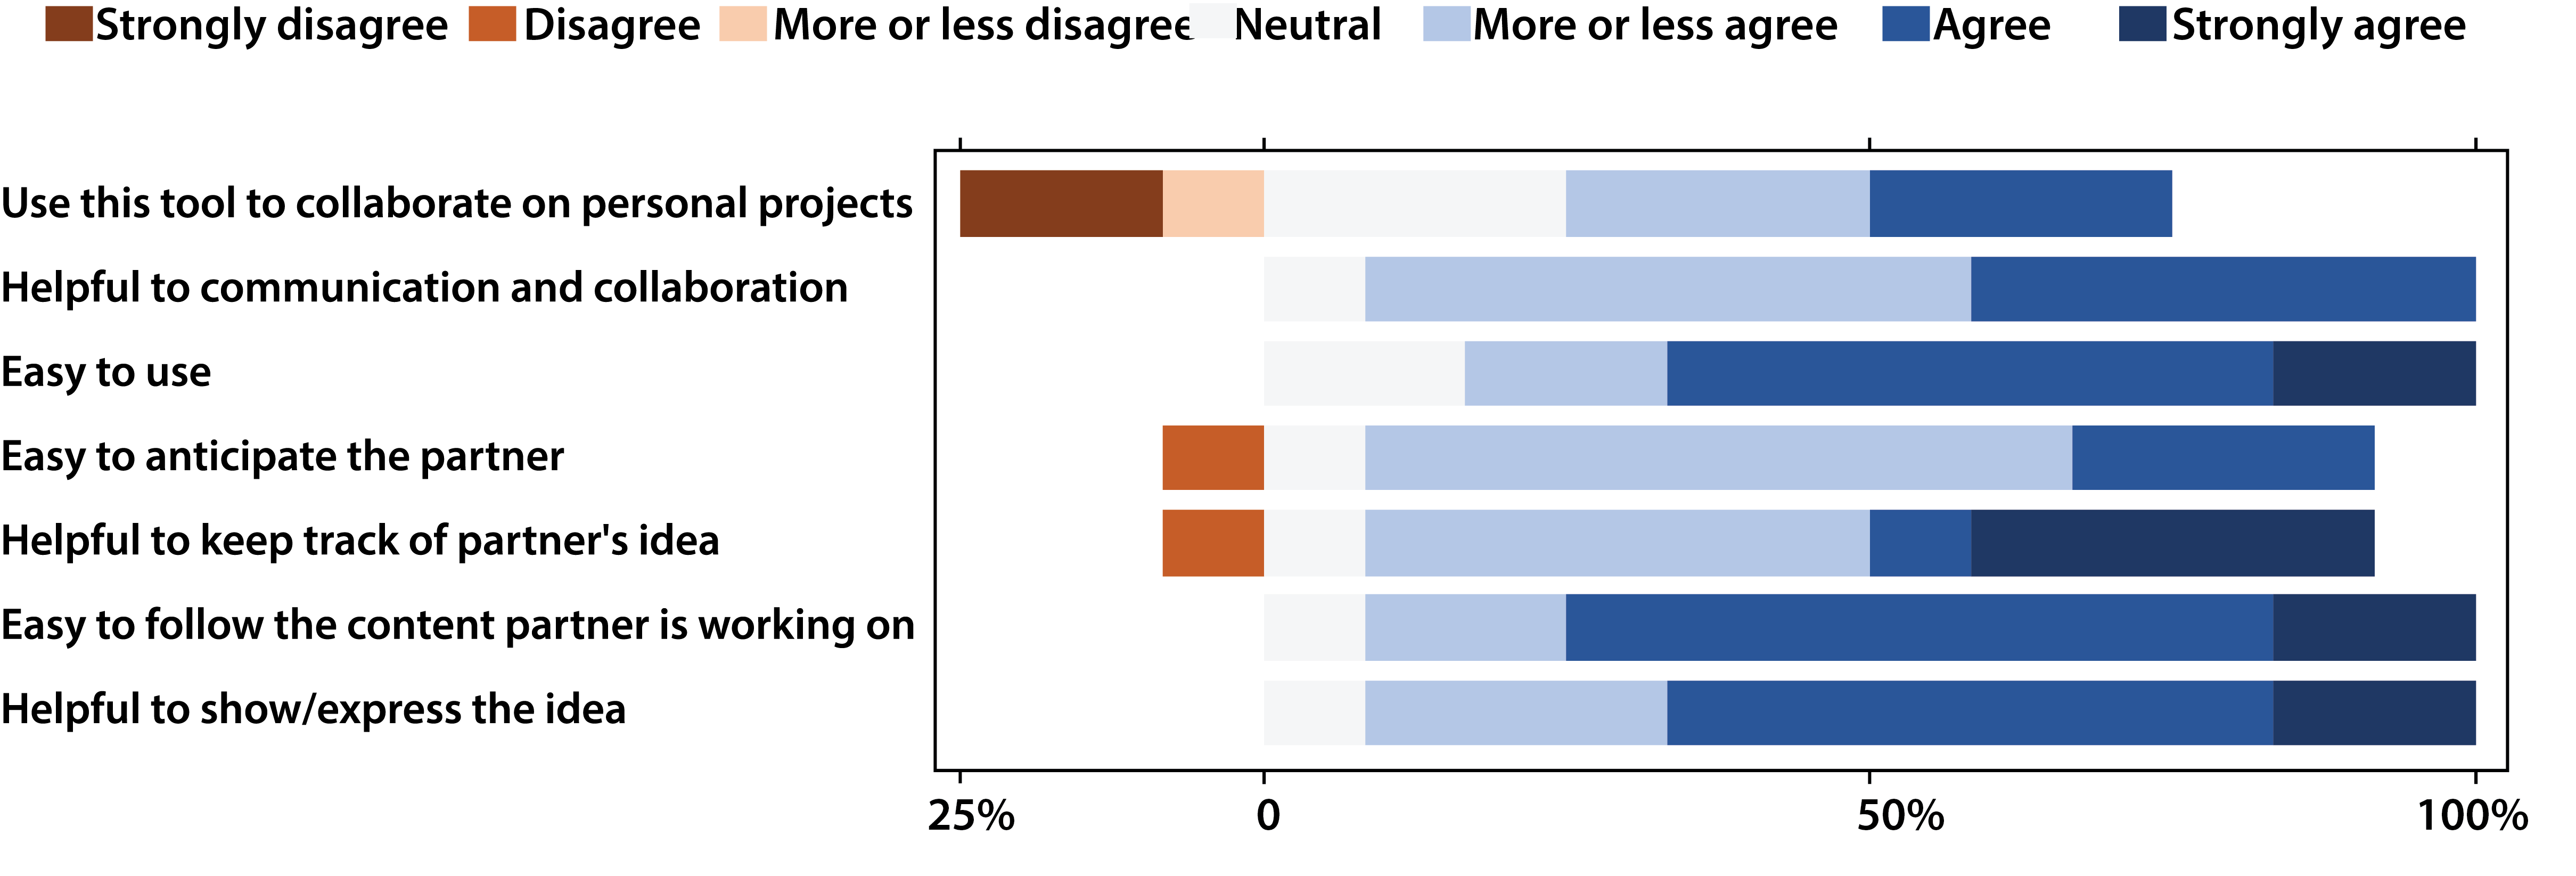
\includegraphics[width=0.98\columnwidth]{usability.png}
 \caption{Agreement distribution of the post-task questionnaire for system usability. The further bars extend to the right, the more users agree.
 }~\label{fig:usability}
\end{figure}
\subsubsection{Usability}
CollaboVR's pipeline was quickly understood by all users. Knowing how to get the permission, conducting free-hand drawing, drawing 3D objects, manipulating the drawing afterwards, and spectating other users. 83.33\% of the participants agreed that the system is easy to use ($M=5.67$, $SD=0.98$). \textit{``It is intuitive to do the drawing in 3D.''} and participant found out the permission strategy design is useful \textit{``Having to get permission to draw is really good at making the environment easier to work in''}(P7,F).
91.67\% of the participants agree that it is helpful to show/express the idea ($M=5.75$, $SD=0.87$). 
\begin{quote}
    There could be merit once you're doing something more complex to 'hey look, this thing, let's do x,y,z...' and that's a lot easier to use this system (P11,M).    
\end{quote}
91.67\% of the participants agree that it is easy to follow the content partner is working on ($M=4.92$, $SD=1.08$).
83.33\% of the participants agree that it is helpful to keep track of partner's idea ($M=5.42$, $SD=1.50$). Partly because the users can \textit{``move themselves easily (P1,M)''}, they can easily follow the partner's drawing and thoughts.
75\% of the participants agree to use this tool to collaborate on personal projects ($M=4.17$, $SD=1.75$). 
\begin{quote}
    That's what I'd use for my own work. It's like a more --not quite as artsy -- business tool. I would use it to get my ideas across to people.(P8,M)
\end{quote}
Similarly, P11(M) thought \textit{``It's totally a great prototyping idea/prototyping system. Can't say it'll replace AutoCAD, but in a few years it will do that.''}

91.67\% of the participants think CollaboVR is helpful to communication and collaboration ($M=5.33$, $SD=0.65$). 
83.33\% of the participants agreed that they can anticipate what the partner would do next ($M=4.92$, $SD=1.08$). P3(F) commented that \textit{``When [...] started to draw the legs for the table, I quickly get his idea about the design of the legs, so he doesn't need to say what kind of legs he wants''}. Participants found it an engaged experience and love to spend more time with friends. \textit{``It's definitely a fun environment, entertaining''}(P7,M).

\begin{table*}
  \centering
  \begin{tabular}{l l l l l l l l l l l}
    % \toprule
    & \multicolumn{2}{c}{Condition1} & \multicolumn{2}{c}{Condition2} & \multicolumn{2}{c}{Condition3} & \multicolumn{2}{c}{ANOVA between C1 and C2} & \multicolumn{2}{c}{ANOVA between C1 and C3} \\
    \midrule
    Performance & 9.67 & (1.53) & 9 & (2) & 5.33 & (2.08) & $F_{(1,5)} = 0.21$ & $p = 0.67$ & $F_{(1,5)} =8.45$ & $p = 0.04*$\\
    Easy to use & 5.67 & (0.98) & 6 & (1.04) & 4 & (1.71) & $F_{(1,23)}=0.65$ & $p=0.43$ & $F_{(1,23)}=8.59$ & $p=0.008*$\\
    % \bottomrule
  \end{tabular}
  \caption{Mean values and standard deviations (in parentheses) for performance and questionnaire results, and ANOVA results between condition1 and other conditions.}~\label{tab:result}
\end{table*}

\subsubsection{User Arrangement}
From table~\ref{tab:result}, there is no significant differences between default user arrangement and mirrored user arrangement for task performance and easy to use. However, 58.33\% of the participants rate this session as the favorite one. Probably because the users have better workspace awareness in this session and they can keep the content and the others in the view together. \textit{``[...] mirrored, it is easy and convenient to communicate with others''} from P3(F) and \textit{``People didn't block my view, and I could see the content clearly''} from P5(M) shared the similar thoughts. 33\% of the participants prefer the default setup most. P2(M) commented \textit{``Because it is comparable to reality.''}. P1(M) had similar opinion. We thought there might be two reasons. One is that some participants have less VR experience. This session is the closest setup comparing to real life. So they can get used to it quickly. The other reason is that mirrored user arrangement will flip other users to the other side of the interactive board. That might lead to the feeling of \textit{``I felt really far away from everyone''}(P7,F).

Then we collect the feedback of the suitable scenario for different user arrangement. Mirrored user arrangement could be user for giving a presentation. P4(M) suggested that because \textit{``You can better control your drawing meanwhile keep an eye on people's reaction through the mirror''}. P5(M) thought about it from a student's view, \textit{``Kind of felt like Khan Academy in 3D vision''}. This is quite consistent to previous work focusing on face-to-face experience. P9(F) thought she can benefit from this setup when brainstorming because no one is blocking the view, \textit{``You can see everybody but you have your own space to work in''}.

\subsubsection{Input Orientations}
From table~\ref{tab:result}, we can see that significant differences were found between different input orientation. Horizontal input orientation has negative impacts on performance and usability. P8(M) commented that \textit{``I think this setup could be really good. Like the tablet. The horizontal board should be slanted more''}. P8(M) is a 3D modeler who used tablet a lot for detailed drawing. So he has more experience with the tablet style input. However, P12(F) felt \textit{``that type of idea works well with a physical tablet''}. The reasons why this setup has negative impacts is probably because most participants are not familiar with such kind of input. We render the same thing on both the personal horizontal board and the shared vertical board. Some user found it difficult to create the correct mapping between the two views. Another reason is that users can rest their elbows on the chair arm when drawing, so they enjoy drawing longer than drawing in the mid-air. Furthermore, participants tended to draw richer details because they felt liking holding a pen. 8.3\% of the participants prefer this setup most and emphasized that \textit{``I had more control over what I was drawing''}. To summarize, horizontal input orientation enables users to draw or write like on a tablet. That encourages the users to draw for a longer time and brings more control to the users. However, users may need more time to get used to the style.

When discussing the suitable scenarios for this setup, P8(M) thought a live demo or presentation could be beneficial from that, especially a time consuming one. He described \textit{``himself giving a presentation to other people looking at the big monitor while an audience was looking at the large monitor-like board''} and \textit{``just want to focus on the board''}. Meanwhile, P11(M) thought it is helpful for collaborative design and suggested us to replace the controller with a pen. We found all of the thoughts are very inspiring.

\section{Discussion, Limitation and Future Work}
The results of our study roughly proved that CollaboVR can be used to communicate with others for non-expert use such as brainstorming and presentation. The system is relatively easy to use and the experience is engaging and entertaining. Participants are willing to hangout with friend in the system. Considering two variance we proposed, mirrored user arrangement has positive but not significant effect on the experience. The users feel the others are synced up with them because of awareness. Horizontal input orientation shows the potential for detailed and long-time experience. However, the learning curve is larger than other setups for user who has less tablet experience. In addition, a physical tablet~\cite{sensel} or a pen~\cite{wu2017dodecapen} as input could be helpful for this setup. 

One limitation of the user study is the diversity of the participants. Most participants are from the department of computer science and the range of the age is not wide enough. The results of our study may not generalized to users such as artist, financial person and older adults. One limitation of the system is that participants found it difficult to track who was speaking. Either visual hints like attaching a speaker to the avatar or mouse tracking will be useful.

In future, we plan to conduct more user study to explore how CollaboVR affect the communication in different scenarios such as presentation and brainstorming. Inspired by P7(F), supporting search engine is an interesting direction too. We also want to investigate other user arrangement and input orientation.

\section{Conclusion}
In this paper we presented CollaboVR - an open-source reconfigurable framework for distributed and co-located multi-user communication in VR. We described the system architecture, two key variables (user arrangement and input orientation), user interface and its implementation. The system was evaluated in a user study showing that user can easily use the system, found it useful for communication and entertaining. We also evaluate the key variables in terms of the performance and usability. Users reported that different combinations of two key variables work differently for different collaborative purposes.

\section{Acknowledgments}
We thank all the volunteers for participating in our experiments and video shoots.

% Your references should be published materials accessible to the
% public.  Internal technical reports may be cited only if they are
% easily accessible (i.e., you provide the address for obtaining the
% report within your citation) and may be obtained by any reader for a
% nominal fee.  Proprietary information may not be cited. Private
% communications should be acknowledged in the main text, not referenced
% (e.g., ``[Robertson, personal communication]'').

%\begin{table}
  %\centering
  %\begin{tabular}{l r r r}
    %% \toprule
    %& & \multicolumn{2}{c}{\small{\textbf{Test Conditions}}} \\
    %\cmidrule(r){3-4}
    %{\small\textit{Name}}
    %& {\small \textit{First}}
      %& {\small \textit{Second}}
    %& {\small \textit{Final}} \\
    %\midrule
    %Marsden & 223.0 & 44 & 432,321 \\
    %Nass & 22.2 & 16 & 234,333 \\
    %Borriello & 22.9 & 11 & 93,123 \\
    %Karat & 34.9 & 2200 & 103,322 \\
    %% \bottomrule
  %\end{tabular}
  %\caption{Table captions should be placed below the table. We
    %recommend table lines be 1 point, 25\% black. Minimize use of
    %table grid lines.}~\label{tab:table1}
%\end{table}

%Place figures and tables at the top or bottom of the appropriate
%column or columns, on the same page as the relevant text (see
%Figure~\ref{fig:figure1}). A figure or table may extend across both
%columns to a maximum width of 17.78 cm (7 in.).

%Captions should be Times New Roman or Times Roman 9-point bold.  They
%should be numbered (e.g., ``Table~\ref{tab:table1}'' or
%``Figure~\ref{fig:figure1}''), centered (if one line) otherwise justified, and placed beneath the figure or table.  Please note that the words ``Figure'' and ``Table'' should
%be spelled out (e.g., ``Figure'' rather than ``Fig.'') wherever they
%occur. Figures, like Figure~\ref{fig:figure2}, may span columns and
%all figures should also include alt text for improved accessibility.

%When possible, include a vector formatted graphic (i.e. PDF or EPS).
%When including bitmaps,  use an image editing tool to resize the image
%at the appropriate printing resolution (usually 300 dpi).

%Quotations may be italicized when \textit{``placed inline''}.

%\begin{enumerate}
%\item Add alternative text to all figures
%\item Mark table headings
%\item Add tags to the PDF
%\item Verify the default language
%\item Set the tab order to ``Use Document Structure''
%\end{enumerate}
%For more information and links to instructions and resources, please
%see: \url{http://chi2016.acm.org/accessibility}.  The
%\texttt{{\textbackslash}hyperref} package allows you to create well tagged PDF files,
%please see the preamble of this template for an example.

%We recommend that you produce a PDF version of your submission well
%before the final deadline.  Your PDF file must be ACM DL
%Compliant. The requirements for an ACM Compliant PDF are available at:
%{\url{http://www.scomminc.com/pp/acmsig/ACM-DL-pdfs-requirements.htm}}.

%Test your PDF file by viewing or printing it with the same software we
%will use when we receive it, Adobe Acrobat Reader Version 10. This is
%widely available at no cost. 

%\section{Acknowledgments}

%Sample text: We thank all the volunteers, and all publications support
%and staff, who wrote and provided helpful comments on previous
%versions of this document.

% Balancing columns in a ref list is a bit of a pain because you
% either use a hack like flushend or balance, or manually insert
% a column break.  http://www.tex.ac.uk/cgi-bin/texfaq2html?label=balance
% multicols doesn't work because we're already in two-column mode,
% and flushend isn't awesome, so I choose balance.  See this
% for more info: http://cs.brown.edu/system/software/latex/doc/balance.pdf
%
% Note that in a perfect world balance wants to be in the first
% column of the last page.
%
% If balance doesn't work for you, you can remove that and
% hard-code a column break into the bbl file right before you
% submit:
%
% http://stackoverflow.com/questions/2149854/how-to-manually-equalize-columns-
% in-an-ieee-paper-if-using-bibtex
%
% Or, just remove \balance and give up on balancing the last page.
%
\balance{}

% BALANCE COLUMNS
\balance{}

% REFERENCES FORMAT
% References must be the same font size as other body text.
\bibliographystyle{SIGCHI-Reference-Format}
\bibliography{sample}

\end{document}

%%% Local Variables:
%%% mode: latex
%%% TeX-master: t
%%% End:
